\documentclass[a4paper,11pt]{article}
\usepackage{amsmath}
\usepackage{epstopdf}
\usepackage{amsfonts}
\usepackage{graphicx}
\usepackage{algorithm,algorithmic}
\usepackage{url}
\usepackage{color}
\usepackage{tikz}
\usepackage{multirow}
\usepackage{verbatim}
%\usepackage{hyperref}
\usepackage{float}
\usepackage{geometry}
\usepackage{indentfirst}
\usepackage{amssymb}
%\usepackage{circuitikz}
\usepackage{array} 
\usepackage{appendix}
\usepackage{float}
\usepackage{graphicx}
\usepackage{url}
\usepackage[colorlinks,linkcolor=blue,anchorcolor=blue,citecolor=blue]{hyperref} % hyper reference to contents
\usepackage{algorithm,algorithmic}
\usepackage{tikz}
\usepackage{suffix}
\usetikzlibrary{arrows,shapes,snakes}





\usepackage[retainorgcmds]{IEEEtrantools}
\geometry{left=3.17cm,right=3.17cm,top=2.54cm,bottom=2.54cm}
\pagestyle{empty}

\newcommand{\opal}{\textsc{OPAL}}
\newcommand{\opalt}{\textsc{OPAL-t }}
\newcommand{\opalcycl}{\textsc{OPAL-cycl}}
\newcommand{\opalmap}{\textsc{OPAL-map }}
\newcommand{\opalenv}{\textsc{OPAL-envelop}}

\newcommand{\mad}{\textsc{mad }}
\newcommand{\madnine}{\textsc{mad9 }}
\newcommand{\madninep}{\textsc{mad9p }}
\newcommand{\madeight}{\textsc{mad8 }}

\newcommand{\classic}{\textsc{classic }}
\newcommand{\hfifepart}{\textsc{H5Part }}
\newcommand{\hfifefe}{\textsc{H5FED }}

\renewcommand{\epsilon}{\varepsilon} 
\renewcommand{\vec}[1]{{\bf #1}} 
\newcommand{\dt}[1]{\frac{\partial #1}{\partial t}}
\newcommand{\dtt}[1]{\frac{\partial^2 #1}{\partial t^2}}
\newcommand{\dtvec}[1]{\frac{\partial {\mathbf #1}}{\partial t}}
\newcommand{\dttvec}[1]{\frac{\partial^2 {\mathbf #1}}{\partial t^2}}
\newcommand{\rot}{\vec{\nabla} \wedge }
\renewcommand{\div}{\vec{\nabla} \cdot }

\def\vec#1{\mathbf{#1}}
\def\vecg#1{\boldsymbol{#1}}
\def\norm#1{\| #1 \|} 
\def\tr{^{\!\top}}

\def\curl{{\bf curl}\,}
\def\curlp{{\rm curl}_p\,}
\def\div{{\rm div}\,}
\def\grad{\nabla}
\def\gradp{\nabla_p}
\def\dotp#1#2{\langle#1,#2\rangle}
\def\eps{\varepsilon}

\newcommand{\mat}[1]{\ensuremath{\boldsymbol{#1}}}
\newcommand{\vect}[1]{\ensuremath{\mathbf{#1}}}
\newcommand{\iprod}[2]{\ensuremath{\langle#1,#2\rangle}}
\newcommand{\abs}[1]{\ensuremath{|#1|}}

\newcommand{\Nedelec}{N\'{e}d\'{e}lec}

\newcommand{\id}[1]{\structure{#1}}

\newcommand {\Co}{{\mathbb{C}}}
\newcommand {\Int}{{\mathbb{Z}}}
\newcommand {\Nat}{{\mathbb{N}}}
%
%
\newcommand {\Hcurl}{{H(\mathbf{curl};\Omega)}}
\newcommand {\Hocurl}{{H_0(\mathbf{curl};\Omega)}}
\newcommand {\Hdiv}{{H(\mathrm{div};\Omega)}}
\newcommand {\Hodiv}{{H_0(\mathbf{div};\Omega)}}
%
\renewcommand {\Re}{{\rm I \kern-2pt R}}
\newcommand{\vc}[1]{\mbox{\boldmath $#1$}}
\newcommand {\RM}[1]{\mathrm{#1}}




\begin{document}
\begin{center}
{\large The Dark Current and Multipacting Simulation Capability of \opal\\ - Modeling, Benchmarking and Applications} \\
{\bf Chuan Wang}, A. Adelmann, Y. Ineichen \\
%\today\\
\end{center}
\begin{abstract}
 Dark current and multipacting phenomena, as observed in accelerator
structures, are usually harmful to the equipment and the beam quality.
These effects need to be suppressed to guarantee stable operation. Large scale
simulations can be used to understand the cause and develop solutions for these
phenomena.
 
We extend OPAL, a parallel framework for charged particle
optics in accelerator structures and beam lines, with the necessary physics models
to simulate multipacting phenomena. This is achieved by adding a Fowler-Nordheim
field emission model and two secondary electron emission models, developed by Furman-Pivi and Vaughan respectively, as well as efficient 3D boundary
geometry handling capabilities to OPAL.

In situations where the electron multiplication is very large, we have to renormalize the simulation particles in order to prevent excessive memory consumption. 

Code to code comparison with the Tech-X physics library and comparison with a non-stationary multipacting  theory for the classic parallel plate geometry will be presented.

Preliminary results on  dark current simulations of the CTF3 electron source and first multipacting simulation in large rf-cavities for compact high intensity Cyclotrons will be  presented. 

\end{abstract}

\begin{figure}[htbp]
\begin{center}
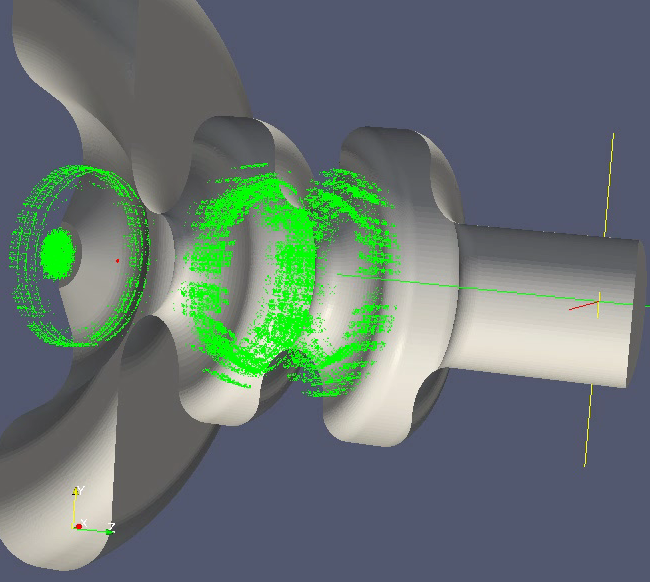
\includegraphics[width=.49\linewidth,angle=0]{Picture1}
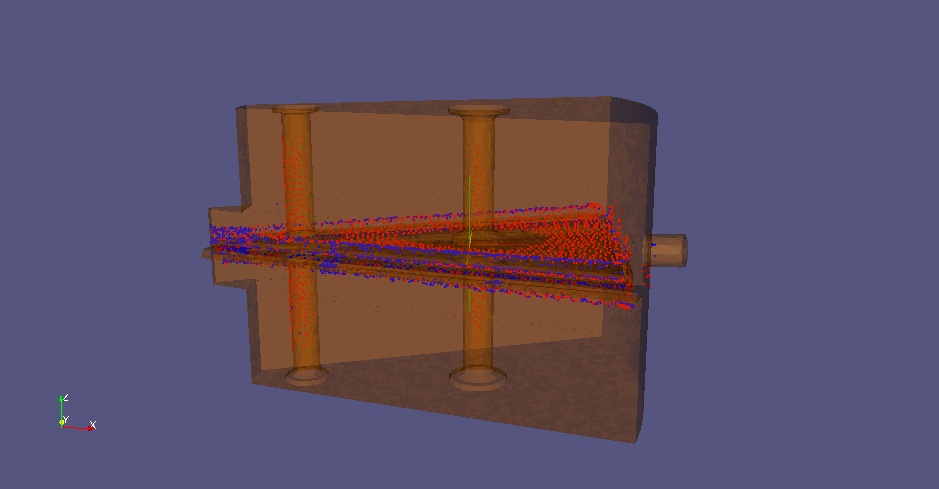
\includegraphics[width=7cm,height=6.43cm,angle=0]{cyclotron_multipacting}
\label{fig:opal-astra-exrms-1}
\end{center}
\end{figure}

{\bf BD-Palaver} 15.2.2011 WBGB 019 14.00 - 15.00
\end{document}


% LocalWords:  Anylitical
